\label {fs-experiments}

To prove the feasibility of the proposed framework we conducted a series of experiments. We show the efficiency and scalability of the distributed streaming dataflow on the top of~\FlameStream\ processing system. Latency and throughput are used as performance metrics. We also demonstrate achieved accuracy using a simple machine learning model. As a dataset, we used an open corpus of news articles from Russian media resource lenta.ru~\cite{lentaru}. This dataset contains about 700 000 documents, which are labeled by one of 90 different topics. In the experiments, we generated a stream consisted of articles from the dataset sorted by the time of publishing.

\begin{figure}[htbp]
  \centering
  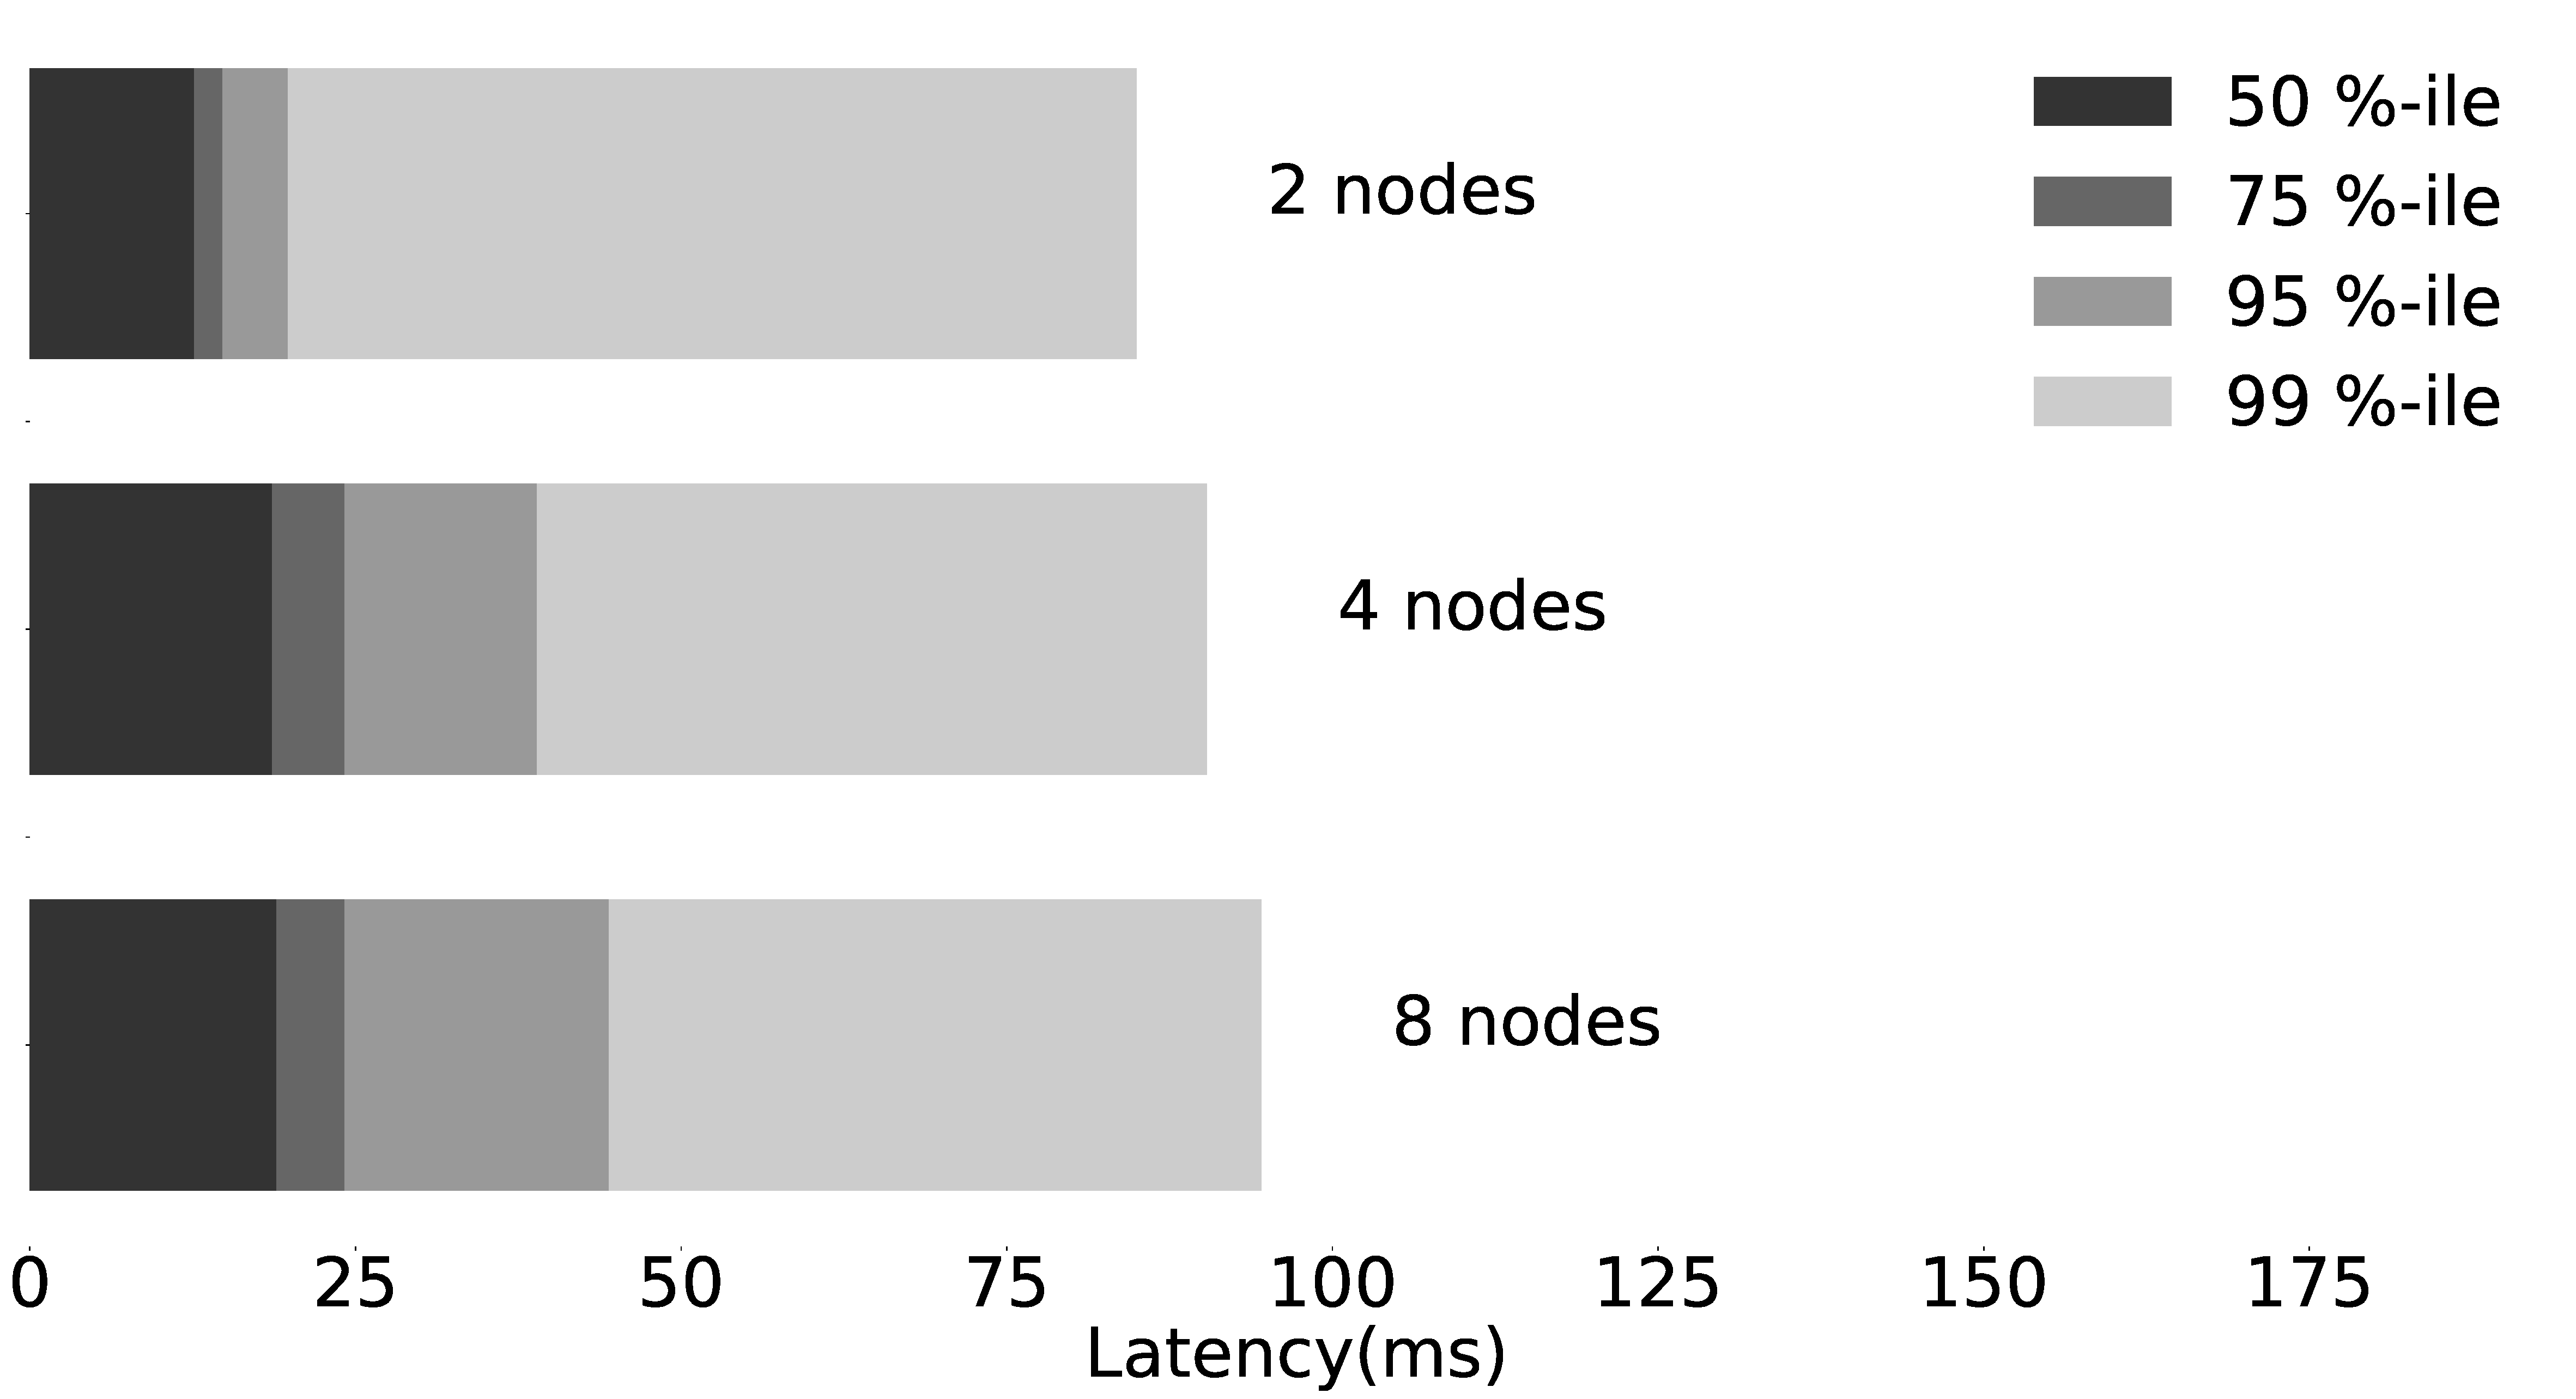
\includegraphics[scale=0.1]{pics/classifier_latencies}
  \caption{Prediction pipeline latencies}
  \label {latencies}
\end{figure}

\subsection{Data flow evaluation}

For evaluation, we deployed FlameStream on clusters, containing 2, 4 and 8 Amazon EC2 small instances with 2 GB of RAM and 1 core CPU. Exactly once guarantee was enabled. We measured throughput that is possible to achieve and the corresponding latency for prediction pipeline\footnote{We took into consideration only the performance of the streaming pipeline without a persistent queue}. The results are shown in Figures~\ref{latencies} and~\ref{throughput}. As we can see, there is a linear trend in throughput, which proves the scalability of the framework. On the other hand, one can observe, that latency increases moderately and keeps under 25 ms for a median and under 100 ms for 99th percentile.

\begin{figure}[htbp]
  \centering
  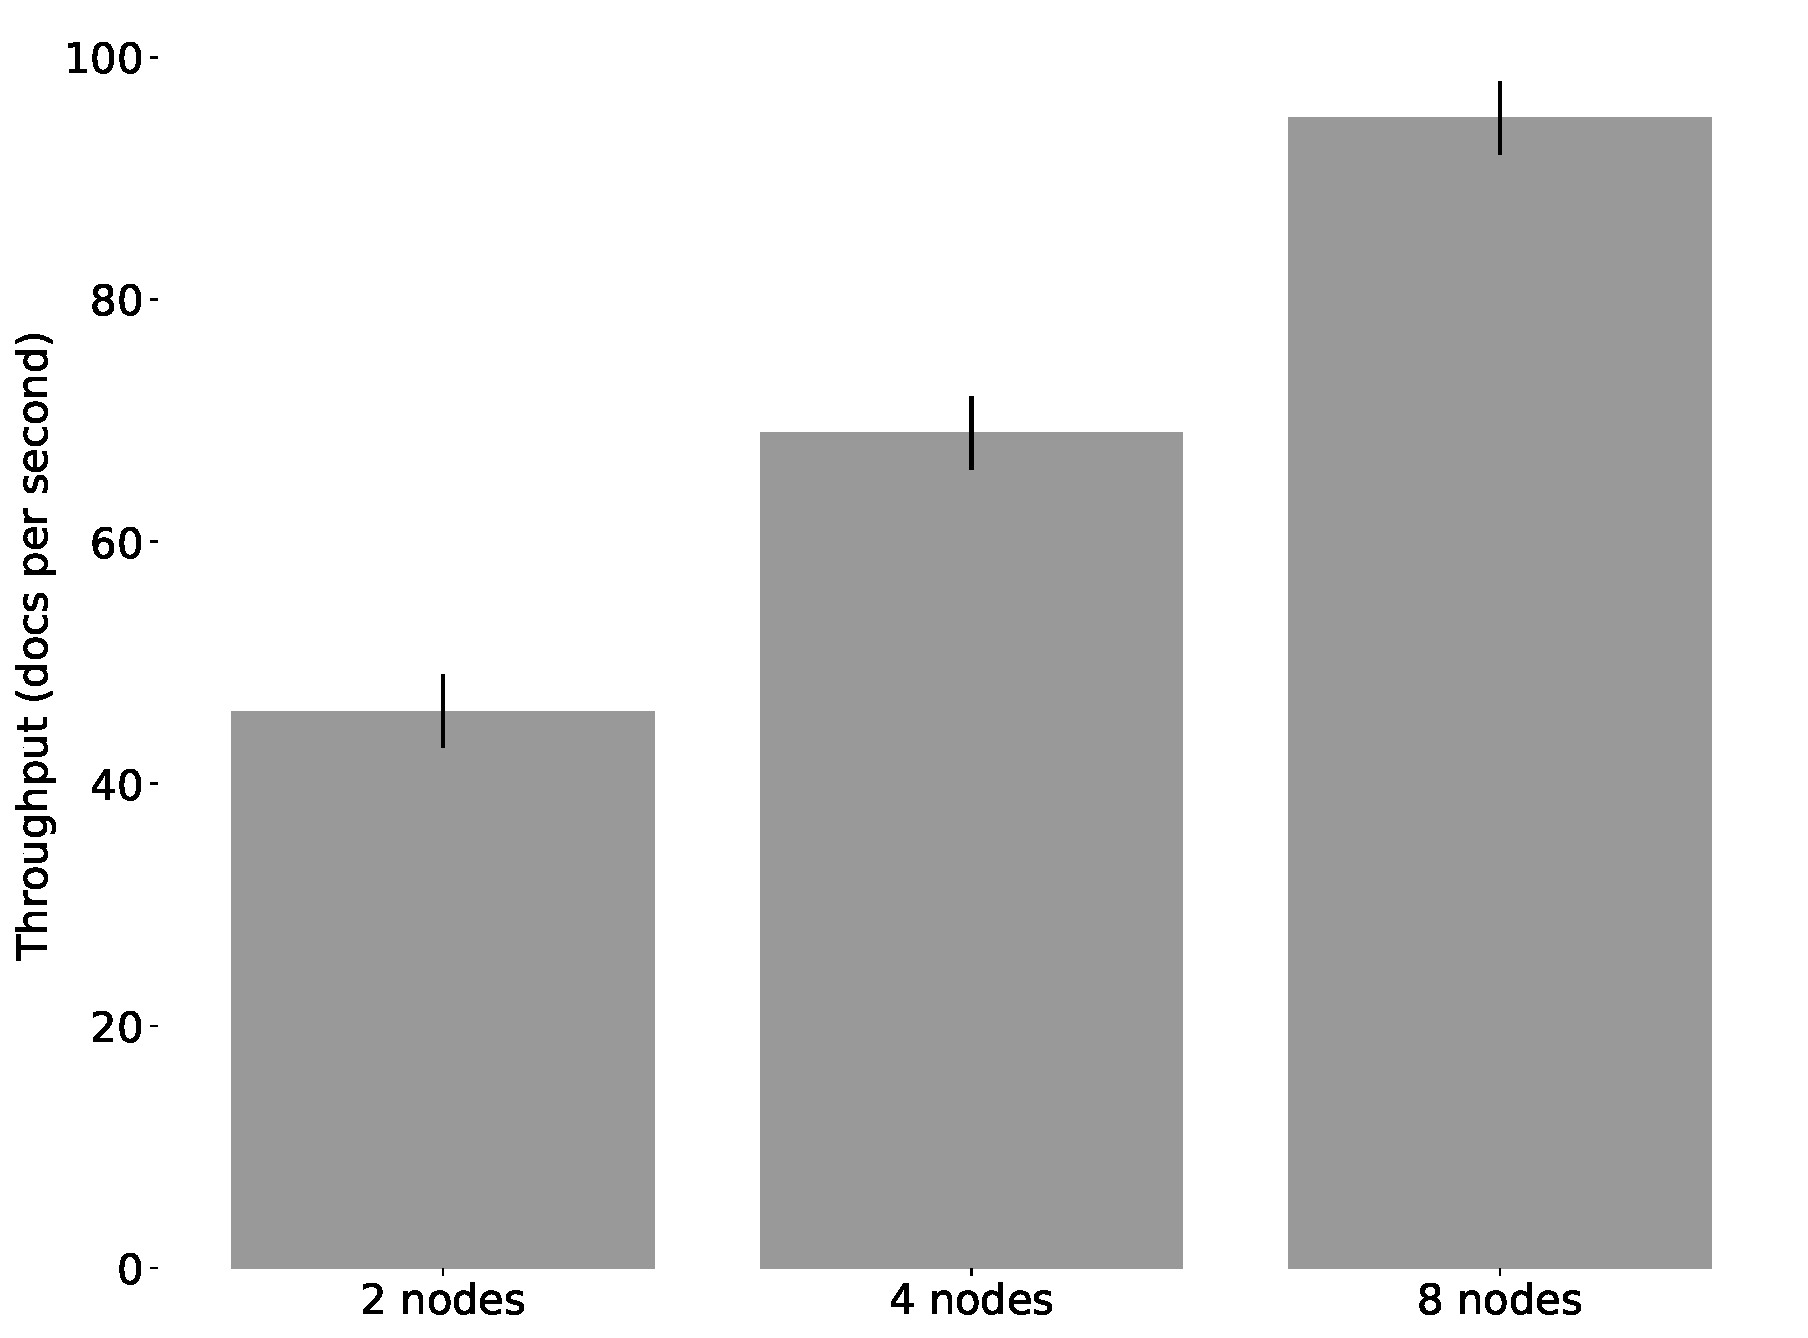
\includegraphics[scale=0.21]{pics/classifier_throughput}
  \caption{Prediction pipeline throughput}
  \label {throughput}
\end{figure}

\subsection{Classifier evaluation}

In order to be efficiently embedded in the proposed data flow, several properties of the machine learning model are desirable:
\begin{itemize}
     \item Small size of the model for storing and updating it in reasonable time and space.
     \item A possibility to update the model with new data.
\end{itemize}

We use Multinomial Logistic Regression as a classification method. Model parameters (weights) are denoted as $W$. The training process is the maximization of the following formula in terms of $W$:

$$ logP(W | X) = \frac{1}{|X|} \sum \limits_{(x, y) \in X} \log \frac{e^{{W_y^T \cdot \; x}}}{\sum \limits_{l = 1}^{k}  e^{{W_{l}^T \cdot \; x}}} - \lambda_1 ||W||_1 - \lambda_2 ||W - W_{prev}||_2 $$ 

$X$ denoted as a training dataset and the number of classes is $k$. Also, $x$ designated as a point in the dataset and $y$ as a label for it. To change the model over time, we use weights that are computed in the previous step -- $W_{prev}$. At the first step, $W_{prev}$ can be provided by a pre-train process.

The first component is the standard softmax function for multiple classes. The second component keeps the $L1$ regularization of the weights, and provides sparsity: with the dictionary of size 560 000, there is only 2\% of non-zero elements in $W$. Hence, the model has a small size -- about 10 Mb. We apply $L2$ regularization as the third component in order to use previous weights for on-the-fly model update.

We compared two approaches to the performance demonstration of the proposed machine learning model. The first one is training on the complete dataset with $\lambda_2 = 0$. We call this approach a {\em static training}. The second one consists in dividing training dataset into relatively small batches and consequent applying MLR with $L2$ regularization to each batch. The latter case demonstrates the behavior of our streaming classification approach. The sizes of train and test datasets are 50 000 and 100 000. The size of batches for the streaming approach is 5 000. Dividing into train and test samples are done uniformly in time: each new text in the stream is put in train or test sample based on a value of a uniformly distributed random variable.

As one can see in Table~\ref{accuracy}, the streaming approach has a slightly lower accuracy in comparison with the static. The achieved value is reasonable considering the number of classes. These results indicate that our framework is able to efficiently solve the text multi-classification problem.

\begin{table}[htbp]
\begin{tabular}{lc}
Method             & Accuracy \% \\
Static training    & 0.647       \\
Streaming training & 0.644         
\end{tabular}
\caption{Accuracy comparison between static and stream training}
\label{accuracy}
\vspace{-7mm}
\end{table}